% Generated by benchmarks/src/utils/make_breakeven_figure.py -- do not hand-edit.
\definecolor{brk0}{HTML}{4285F4}
\definecolor{brk1}{HTML}{EA4335}
\definecolor{brk2}{HTML}{FBBC05}
\definecolor{brk3}{HTML}{EDA100}
\definecolor{brk4}{HTML}{E87BA4}
\definecolor{brk5}{HTML}{008300}
\definecolor{brk6}{HTML}{34A853}
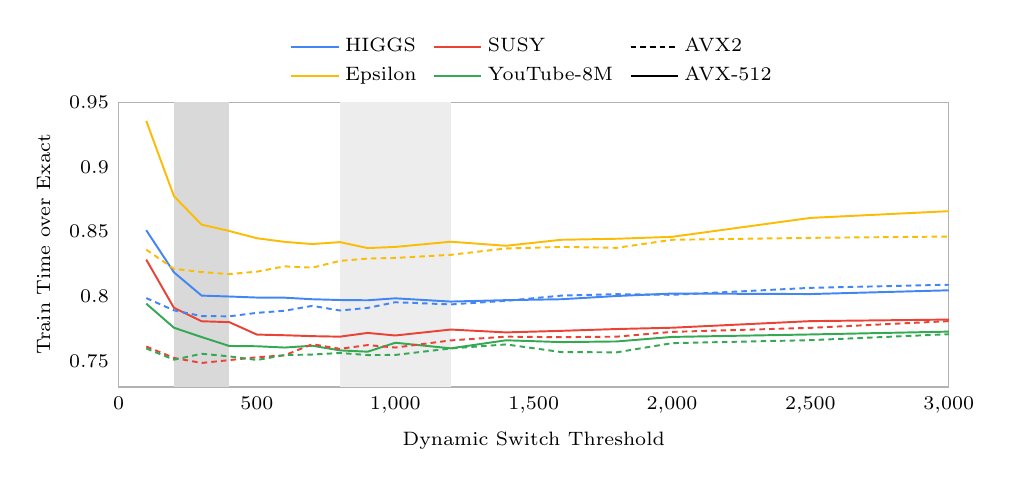
\begin{tikzpicture}
\begin{axis}[width=\linewidth, height=5.2cm, xmode=normal, xmin=0, xmax=3000,
  ymin=0.73, ymax=0.95, xtick={0,500,1000,1500,2000,2500,3000}, log ticks with fixed point,
  xlabel={Dynamic Switch Threshold},
  ylabel={Train Time over Exact}, tick label style={font=\scriptsize},
  label style={font=\scriptsize}, grid=none, axis line style={gray!60}, tick style={draw=none},
  every axis plot/.append style={line width=0.7pt, mark size=1.1pt},
  legend style={font=\scriptsize, draw=none, fill=none, at={(0.5,1.02)}, anchor=south, legend columns=3,
    /tikz/every even column/.append style={column sep=4pt}}, legend cell align=left,
  scaled x ticks=false, scaled y ticks=false, yticklabel style={/pgf/number format/fixed, /pgf/number format/precision=2}]
\fill[gray!14] (axis cs:800,0.73) rectangle (axis cs:1200,0.95);
\fill[gray!30] (axis cs:200,0.73) rectangle (axis cs:400,0.95);
\addplot[gray!70, dashed, line width=0.6pt, forget plot] coordinates {(0,1) (3000,1)};
\addplot[color=brk0, mark=none, solid, forget plot] coordinates {(100,0.8511) (200,0.8186) (300,0.8006) (400,0.7999) (500,0.7991) (600,0.7990) (700,0.7978) (800,0.7972) (900,0.7970) (1000,0.7985) (1200,0.7960) (1400,0.7971) (1600,0.7978) (1800,0.8003) (2000,0.8022) (2500,0.8018) (3000,0.8047) (3500,0.8071) (4000,0.8117) (4500,0.8121) (5000,0.8123) (6000,0.8111) (7000,0.8127) (8000,0.8200) (9000,0.8127) (10000,0.8158)};
\addplot[color=brk1, mark=none, solid, forget plot] coordinates {(100,0.8284) (200,0.7912) (300,0.7808) (400,0.7801) (500,0.7705) (600,0.7700) (700,0.7693) (800,0.7689) (900,0.7718) (1000,0.7698) (1200,0.7744) (1400,0.7722) (1600,0.7734) (1800,0.7748) (2000,0.7758) (2500,0.7809) (3000,0.7821) (3500,0.7855) (4000,0.7865) (4500,0.7861) (5000,0.7877) (6000,0.7918) (7000,0.7959) (8000,0.7980) (9000,0.8057) (10000,0.8013)};
\addplot[color=brk2, mark=none, solid, forget plot] coordinates {(100,0.9355) (200,0.8774) (300,0.8554) (400,0.8505) (500,0.8449) (600,0.8421) (700,0.8404) (800,0.8419) (900,0.8373) (1000,0.8382) (1200,0.8422) (1400,0.8391) (1600,0.8437) (1800,0.8445) (2000,0.8460) (2500,0.8606) (3000,0.8658) (3500,0.8510) (4000,0.8538) (4500,0.8596) (5000,0.8574) (6000,0.8614) (7000,0.8637) (8000,0.8669) (9000,0.8675) (10000,0.8695)};
\addplot[color=brk6, mark=none, solid, forget plot] coordinates {(100,0.7944) (200,0.7758) (300,0.7686) (400,0.7617) (500,0.7615) (600,0.7605) (700,0.7619) (800,0.7583) (900,0.7573) (1000,0.7642) (1200,0.7599) (1400,0.7661) (1600,0.7647) (1800,0.7652) (2000,0.7687) (2500,0.7706) (3000,0.7728) (3500,0.7738) (4000,0.7744) (4500,0.7761) (5000,0.7774) (6000,0.7768) (7000,0.7822) (8000,0.7848) (9000,0.7848) (10000,0.7875)};
\addplot[color=brk0, mark=none, dash pattern=on 2pt off 1.5pt, forget plot] coordinates {(100,0.7987) (200,0.7892) (300,0.7848) (400,0.7846) (500,0.7873) (600,0.7889) (700,0.7927) (800,0.7891) (900,0.7911) (1000,0.7955) (1200,0.7938) (1400,0.7966) (1600,0.8006) (1800,0.8017) (2000,0.8012) (2500,0.8066) (3000,0.8090) (3500,0.8088) (4000,0.8116) (4500,0.8150) (5000,0.8110) (6000,0.8170) (7000,0.8175) (8000,0.8197) (9000,0.8159) (10000,0.8218)};
\addplot[color=brk1, mark=none, dash pattern=on 2pt off 1.5pt, forget plot] coordinates {(100,0.7613) (200,0.7525) (300,0.7486) (400,0.7508) (500,0.7530) (600,0.7545) (700,0.7631) (800,0.7595) (900,0.7624) (1000,0.7605) (1200,0.7660) (1400,0.7689) (1600,0.7685) (1800,0.7689) (2000,0.7726) (2500,0.7757) (3000,0.7809) (3500,0.7822) (4000,0.7843) (4500,0.7907) (5000,0.7936) (6000,0.7936) (7000,0.7965) (8000,0.8010) (9000,0.8021) (10000,0.8008)};
\addplot[color=brk2, mark=none, dash pattern=on 2pt off 1.5pt, forget plot] coordinates {(100,0.8361) (200,0.8213) (300,0.8188) (400,0.8172) (500,0.8191) (600,0.8232) (700,0.8222) (800,0.8274) (900,0.8292) (1000,0.8297) (1200,0.8321) (1400,0.8370) (1600,0.8382) (1800,0.8375) (2000,0.8437) (2500,0.8452) (3000,0.8462) (3500,0.8520) (4000,0.8578) (4500,0.8527) (5000,0.8579) (6000,0.8597) (7000,0.8633) (8000,0.8666) (9000,0.8686) (10000,0.8710)};
\addplot[color=brk6, mark=none, dash pattern=on 2pt off 1.5pt, forget plot] coordinates {(100,0.7598) (200,0.7511) (300,0.7557) (400,0.7537) (500,0.7509) (600,0.7547) (700,0.7551) (800,0.7563) (900,0.7547) (1000,0.7548) (1200,0.7598) (1400,0.7629) (1600,0.7570) (1800,0.7568) (2000,0.7639) (2500,0.7662) (3000,0.7708) (3500,0.7699) (4000,0.7737) (4500,0.7737) (5000,0.7719) (6000,0.7745) (7000,0.7828) (8000,0.7793) (9000,0.7798) (10000,0.7824)};
\addlegendimage{color=brk0, solid, line width=0.7pt, mark=none}
\addlegendentry{HIGGS}
\addlegendimage{color=brk1, solid, line width=0.7pt, mark=none}
\addlegendentry{SUSY}
\addlegendimage{color=black, dash pattern=on 2pt off 1.5pt, line width=0.7pt, mark=none}
\addlegendentry{AVX2}
\addlegendimage{color=brk2, solid, line width=0.7pt, mark=none}
\addlegendentry{Epsilon}
\addlegendimage{color=brk6, solid, line width=0.7pt, mark=none}
\addlegendentry{YouTube-8M}
\addlegendimage{color=black, solid, line width=0.7pt, mark=none}
\addlegendentry{AVX-512}
\end{axis}
\end{tikzpicture}
